\documentclass[12pt]{article}

\usepackage{sbc-template}

\usepackage{graphicx,url}
\usepackage{authblk}

\usepackage[utf8]{inputenc}  
% UTF-8 encoding is recommended by ShareLaTex
\sloppy

\title{Team Description Paper of \\
Indian Institute of Technology Kharagpur for IARC}

\author[]{Palak Harwani}
\author[]{Shubhika Garg}
\author[]{Akshat Pandya}
\author[]{Vidit Goel}
\author[]{Aditi Singh}
\author[]{Aman Modi}
\author[]{Gaurav Suryawanshi}
\author[]{Akshay Jain}
\author[]{Anvee Naik}

\affil[]{Students\\ Indian Institute of Technology, Kharagpur}



\renewcommand\Authands{ and }

\begin{document}
\maketitle
\begin{abstract}

\begin{center}\textbf{ABSTRACT}\end{center}
This paper describes the current preparation strategy of Aerial Robotics Kharagpur,
participating in IARC Mission 7 2018. Our main goal includes robust, indoor 
localization in GPS denied environments supported by optical flow sensors. 
Other features like ground i-robots detection and differentiation between the 
target bots and patrol bots is also discussed, followed by a brief description 
of the herding AI algorithm to be used.
\end{abstract}
\section{INTRODUCTION}
Our research group, Aerial Robotics Kharagpur, started in January 2015 with IARC 
being the prime target. Hence we started on with the problem statement of IARC 
mission 7. Our team was organized into two major domains, which are "controls" 
and "software". Keeping Robot Operating System (ROS) as the base we developed 
our simulation environment in ROS and Gazebo in order to speed up the software 
development and testing while the hardware gets ready. As mission 7 is based 
indoor, hence we made April Tags based indoor true value setup. We have a website[18] 
and a GitHub Organization[19].
\section{SIMULATION}
Gazebo, an open source robotics simulator is being used to simulate the robot along with its mathematical, physical and visualization model.It also emulates the environment with the physics and other interactive robots.We have made ROS plugin for the behaviour of i-robots, whereas the quadcopter model,
is made on top of hector\_gazebo, supported by JSBSim, ArduCopter, RotorS,MAVROS,ardupilot\_sitl\_gazebo plugin. For simulations on Pixhawk, we used PX4 SITL after interfacing it with ROS.
\begin{center}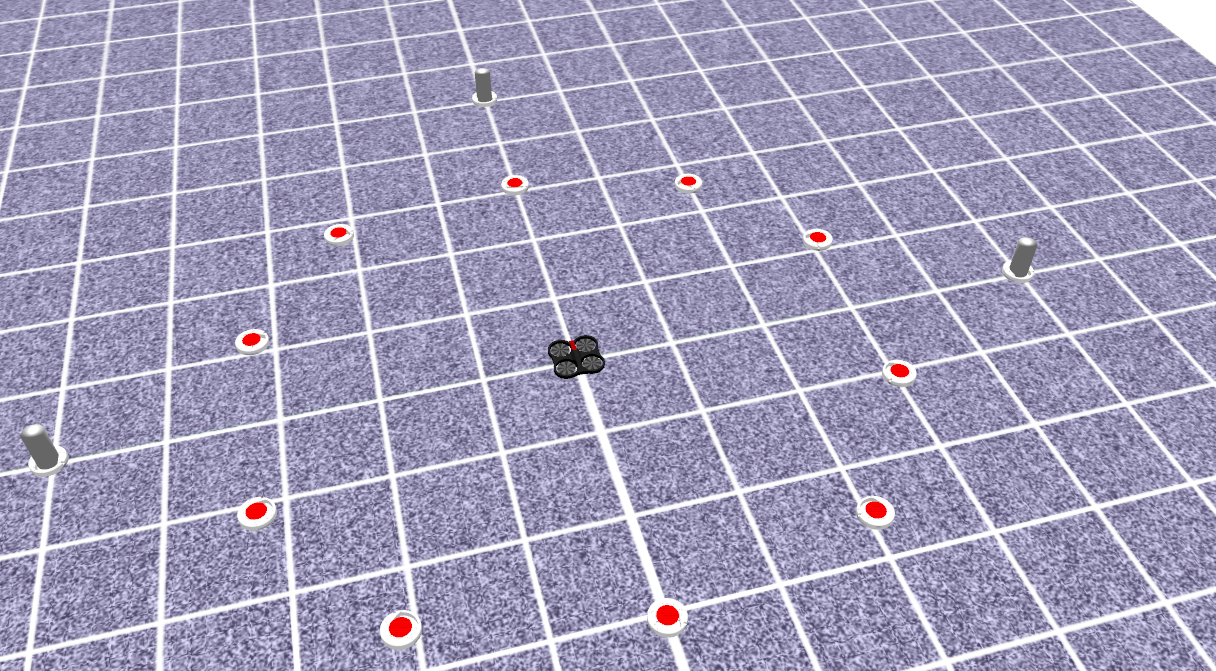
\includegraphics[scale=0.15]{sim} \\
\textbf{Figure 1. Gazebo Simulator.}\end{center}

\section{OVERALL SYSTEM DESIGN}
\begin{center}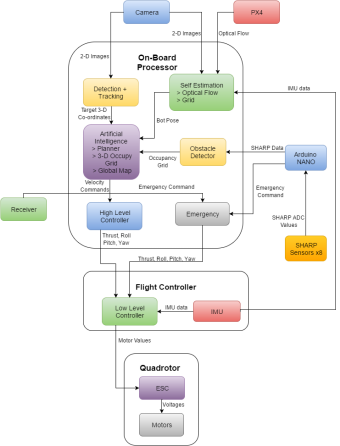
\includegraphics[scale=0.5]{image22} \\
\textbf{Figure 2. System design}\end{center} \\

\section{LOCALIZATION}
We propose a monocular visual localization algorithm over grid-lines algorithm for indoor  localization  of  Micro  Aerial Vehicles  (MAVs)  that  is  accurate  and  computationally  fast for  real-time  on-board  processing. The algorithm  explicitly models  the  grid-lines  and  uses  probabilistic  clustering  and labeling  method  to  fit  observed  grid-lines  to  the  model.  A Random sample consensus (RANSAC) method is used to detect outliers and reject the false positive lines before fitting the model.It performs a five degree of freedom (5DoF) localization (position along X, Y, Z axis, roll and pitch) relative to  the  grid-based  floor  in  a  two-step  sequential  process.  The first step involves localizing the MAV within a unit grid cell. Since a grid is a 2D plane of repeating unit cells (rectangles),the  unit  cells  cannot  be  differentiated  from  each  other  when only a partial grid is visible. Hence, the relative positions are integrated using a winner take all (WTA) method in the second stage  to  determine  the  position  estimate  over  the  grid-based floor.\\
In cases where grid localisation cannot work, that is when the hex-rotor is at very low heights, we use optical flow for localisation.The concept of 2D vector field where each vector is a displacement vector showing the movement of points from first frame to second is used.
\subsection{Grid Localization}
 In our implementation, we use Hough Transform. Since we can filter out the false positives (outliers), we use Hough Transform  with  threshold  parameters  that  allow  for  more false  positives  than  false  negatives.  Each  line  is  represented by  a  two-element  ordered  set(\rho;\theta).\  $\rho$  is  the  perpendicular distance between the line and the coordinate origin (0;0) (top-left  corner  of  the  image)  in  pixels.  While $\theta$ \  is  the  angle  in radians,  the  normal  to  the  line  makes  with  the X axis  of image.   Let $L_r_a_w$= \{ ($\rho$; $\theta$) \in \  $R^2$ | \rho \geq 0;\ -\pi \ \leq \theta < \ \pi \ \} \   $be the set of all the detected lines.$ 
 \\ 
 $L_r_a_w$ = $L_i_n_l_i_e_r_s$ \bigcup \  $L_o_u_t_l_i_e_r_s$ \ , where $L_i_n_l_i_e_r_i_s$  a  set  of  lines  that  belong  to  grid-lines,  and $L_o_u_t_l_i_e_r$ \ is  the set of lines which are not a part of the grid-lines, as detected from the image. Hence a line is represented by a point in (\rho;\theta) \ space.
\subsubsection{Detecting the Grid}
We  use the  linear  relationship  between $\rho$ and $\theta$ for  a  set  of  parallel  lines,  and  perform  a  Random  Sampling
Consensus  (RANSAC)  with  a  2D  linear  model  on  the  set of  detected  lines $L_r_a_w$ .  RANSAC  is  performed  twice  without replacement  to  get  two  best  fit  inliers  to  the  linear  model , hence  two  best  sets  of  parallel  lines  from $L_r_a_w$ .  Further,  the set  of  parallel  lines  (ordered  set  of ($\rho$ ; $\theta$ )),  with  arithmetic mean  of $\theta$ closer  to 0 is  denoted  as $L_l_o_n_g$ and  that  closer  to $\pi$/2 is denoted as $L_l_a_t$ . Hence, the filtered set of lines $L_f_i_l$ , that contains  only  those  detected  lines  which  belong  to  the  grid-lines (two sets of parallel lines with separation of around $\pi$/2 in  mean $\theta$ is  generated  as $L_f_i_l$ = \ $L_l_o_n_g$ \bigcup \ $L_l_a_t$
\\
We use univariate kernel density estimation (KDE)to  estimate  the  probability  density  of $\rho$ in $L_l_a_t$ and $L_l_o_n_g$ individually, as given by
\begin{equation*}
$f_b($\rho$)$ \  = \frac{1}{nb} $\sum\limits_{i=1}^{n}$ K\left(\frac{\rho - \rho_i}{b}\right)
\end{equation*} \\
\begin{center}
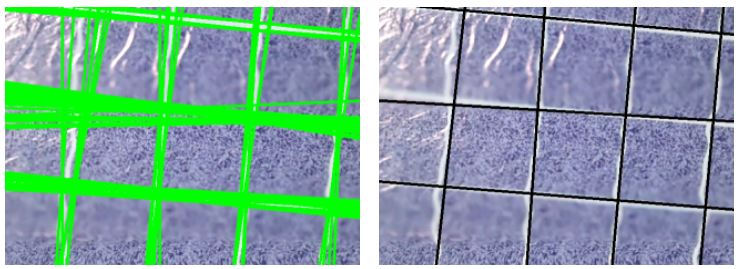
\includegraphics[scale=0.6]{grid2}\\
\textbf{Grid Line Detection}
\end{center}
\subsubsection{Orientation and Cell Localisation}
\begin{itemize}
    \item   In  the $\rho$ ; $\theta$ \ space,  the slopes of the linear curves $m_l_a_t$ and $m_l_o_n_g$ , joining the ordered sets  of  parallel  lines  in $L_l_a_t$ and $L_l_o_n_g$ are  related  to roll ( $\alpha$ ) and pitch ( $\beta$ ) respectively as \\ 
    $\alpha$ = \ $tan^-^1(m_l_a_t)$ \times \  $\epsilon_\alpha$ + $\epsilon_c_\alpha$ \\
    $\beta$ = \ $tan^-^1(m_l_o_n_g)$ \times \  $\epsilon_\beta$ + $\epsilon_c_\beta$ \\ 
    where $\epsilon_\alpha$, $\epsilon_c_\alpha$, $\epsilon_\beta$ and $\epsilon_c_\beta$ are constants obtained from camera calibration.
    \item  We  consider  the  distance  ($s_Y$) between  each  longitudinal line of the grid-based floor and the camera position along $Y_W$ axis.  The  line  to  the  immediate  positive $Y_W$ direction,  with respect to the camera position is indexed as i = 0.
    \item The projection of any line of magnitude c in $Y_W$ axis with camera position as the origin is given by g(c)

    $\textit{g(c)} = \left(\frac{{c \times cos(\phi_Y) \times f}}{cos(\delta)\times h}\right)$ 
   \paragraph{}    \item Squared L2 error cost function is used to estimate sub cell position and height based on observed \rho .
\end{itemize}
\begin{center}
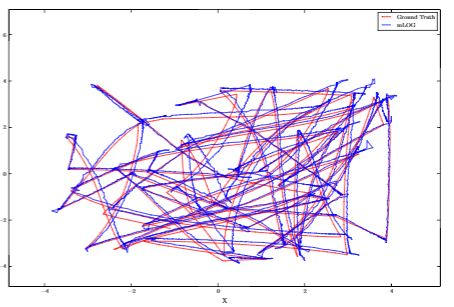
\includegraphics[scale=0.6]{grid}\\
\textbf{Localization and True Value}
\end{center}}
\subsubsection{Grids Localization}
Let $\sigma_k^Y$ be  the  position  within $u_k$ unit  cell  and $p^k_Y$ be  the position  of  the  MAV  with  respect  to  an  initial  position  over the grid-based floor at $k^t^h$ frame. Hence we have \\
$u_k$ = $\left(\frac{p^k_Y}{m_Y}\right)$ \\
At $(k + 1)^t^h$ frame, the new sub-cell position $\sigma^k^+^1_Y$ , might be from $u_k_-_1$ ,$u_k$ or $u_k_+_1$ unit cell, considering the maximum MAV speed is limited. Hence three possible position of the MAV at $(k + 1)^t^h$ frame are $P_Y$ = $\{(p_Y_- 1);(p_Y);(p_Y + 1)$ \\
where $p_Y$ = $p^k_Y$ + $\sigma^k^+^1_Y$ - $\sigma^k_Y$. The MAV’s new position $(p^k^+^1_Y)$ is given by a winner take all (WTA) scheme, decided by $p^k^+^1_Y$ = $argmin(p^k_Y - p^'$$_Y )^2$ 
\section{GROUND ROBOT DETECTION}
    \subsection{Using Downward Facing Camera}
    	 \subsubsection{Preprocessing the Image}
            The images from the video feed consist of a lot of noise due to the patterns present between the grid and also due to the constant movement of our MAV, to remove this noise we use multiple applications of Gaussian blur.
        \subsubsection{Circle Detection}
        One of the most apparent features of the ground robots is that they appear circular when seen from the top, we use this property for detection.
            \begin{itemize}
                \item To obtain circles in the image we applied Canny edge detection algorithm on the smoothened image and then processed the obtained image using hough transform for circle detection.
                \item To get an approximate pixel radius for the circles present in the image we performed a simple world to pixel distance transform using the camera parameters.
Hence we found the ground robots present in a frame of the video feed.\\
            \end{itemize} 
    \begin{center}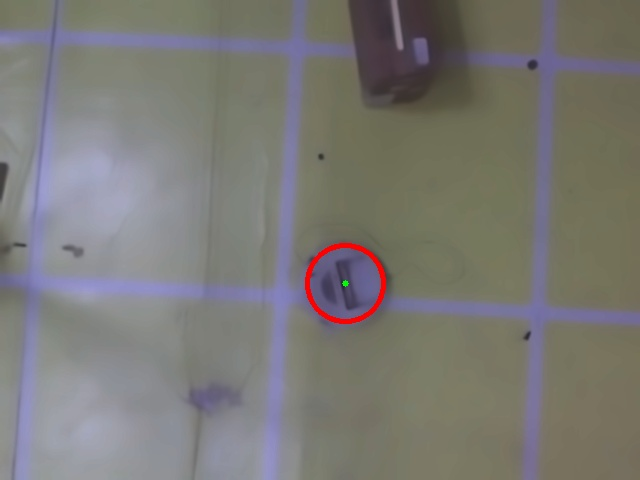
\includegraphics[scale=0.2]{Pic2} \\
    \textbf{Bot Detection using Circle Detection for downward facing camera}\end{center}
       \subsubsection{Colour Thresholding}
       		\begin{itemize}
       			\item Another prominent feature of the ground robots is the red or green colour present on them.
				\item To detect these we converted the image into HSV colour scale and did binarization using colour thresholds, thus obtaining the required ROIs in the binary image.
				\item These ROIs were then differentiated from each other using contour detection. 
       		\end{itemize}
       	\subsubsection{Position and Orientation Estimation}
       		\begin{itemize}
       			\item We obtain the pixel coordinates of the centre of the ground robots present in a particular frame by merging the data from the above mentioned techniques.
       			\item These pixel coordinates are transformed into world coordinates with respect to our MAV and these are then translated into the global frame by using our current position feedback obtained from grid localisation. Thus we get the position of the robot.
       			\item  The orientation of any robot is obtained by analysing the position data over 5 consecutive frames and mapping the change in the coordinates.
       		\end{itemize}  
    \subsection{Using Front Facing Camera}
    	\subsubsection{Color Thresholding}       
			\begin{itemize}
        		\item The detection of each ground robot will be done using color             thresholding. A color threshold for each of red and blue bots along with the grid axis is done. Image subtractions initially removes the grid from the feed so that bot detection becomes easier.
        	\end{itemize}
		\subsubsection{Detection}
			\begin{itemize}           
				\item Contour detection is used to detect the the image cordinates of a particular bot. 
				\item Image is first converted into canny from which contours are detected         
			\end{itemize}            
		\subsubsection{Position estimation}        
			\begin{itemize}            
				\item Pixel coordinates are then converted into real world coordinates using perspective transformation.             
				\item  First the pixels are converted into camera cordinates and then to world cordinates. Due to the presence of Gimbal rotation matrix of the camera does not change. 
				\item With given camera coordinates, translation matrix can be easily predicted which gives the output in world frame given pixel cordinates

			\end{itemize}     
			\begin{center}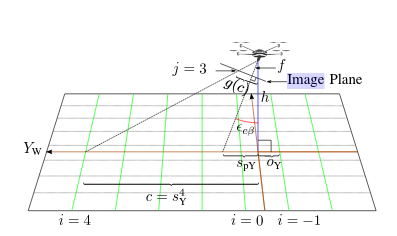
\includegraphics[scale=0.44]{trig} \\
    \textbf{Trignometric pose estimation from front camera}\end{center} 
		\subsubsection{Orientation  Estimation}            
			\begin{itemize}       
				\item Orientation is estimated by comparing the last 5 frames data 		which is stored.                         
			\end{itemize}
			
\section{ACTIVE LOCALISATION}
	\subsection{Tracking of Robots}
The dynamics explained above tell us that it is a non linear system. Also Gaussian noise is introduced in the system at frequent intervals of time. Hence, we use Extended Kalman filter for predicting and updating states of the bot.

\[ s_k = f(s_{k-1}, u_{k-1})\] 

\[
s_k=
  \begin{bmatrix}
    x_k \\
    y_k \\
    \theta_k
  \end{bmatrix}
\]

\[
f=
  \begin{bmatrix}
    u_x_{k-1} + v\delta t cos(\theta_{k-1})\\
    u_y_{k-1} + v\delta t sin(\theta_{k-1}) \\
    \theta_{k-1}
  \end{bmatrix}
\]

\[
F=
  \begin{bmatrix}
    1 && 0 && 0\\
    0 && 1 && 0\\
    0 && 0 && 1\\
  \end{bmatrix}
\]



Error Co-variance matrix P is mathematically found by calculating co-variance of state.
State equations considered are mentioned below
 \[
 x_{k} =  x_{k-1} + v\delta t cos(\theta_{k-1})\]
 \[y_{k} =  y_{k-1} + v\delta t sin(\theta_{k-1})\] 
 \[\theta_{k} =   \theta_{k-1}\]
Result comes out to be
\[ P_{k} = P_{k-1} + Q\]
 
\[
Q =
  \begin{bmatrix}
    3v^2(0.5 + e^{-2\sigma^2}cos(\theta) - e^{-\sigma^2}cos(\theta)^2 && 3v^2sin(2\theta)e^{-\sigma^2}(e^{-\sigma^2} - 1)0.5 && v\sigma^2 sin(\theta) e^{-\sigma^2}0.5\\
    3v^2sin(2\theta)e^{-\sigma^2}(e^{-\sigma^2} - 1)0.5 && 3v^2(0.5 + e^{-2\sigma^2}cos(\theta) - e^{-\sigma^2}sin(\theta)^2 &&  v\sigma^2 cos(\theta) e^{-\sigma^2}0.5\\
    v\sigma^2 sin(\theta) e^{-\sigma^2}0.5 &&  v\sigma^2 cos(\theta) e^{-\sigma^2}0.5 && \sigma^2\\
  \end{bmatrix}
\]

Q is a symmetric matrix.\\

\subsection{Predict Stage}
\[ x = f\]
\[ P_{k} = P_{k-1} + Q\]
As we are getting a noise after every 5 seconds we will be increasing the sigma by 10 degree after every 5 sec.\\

\begin{center}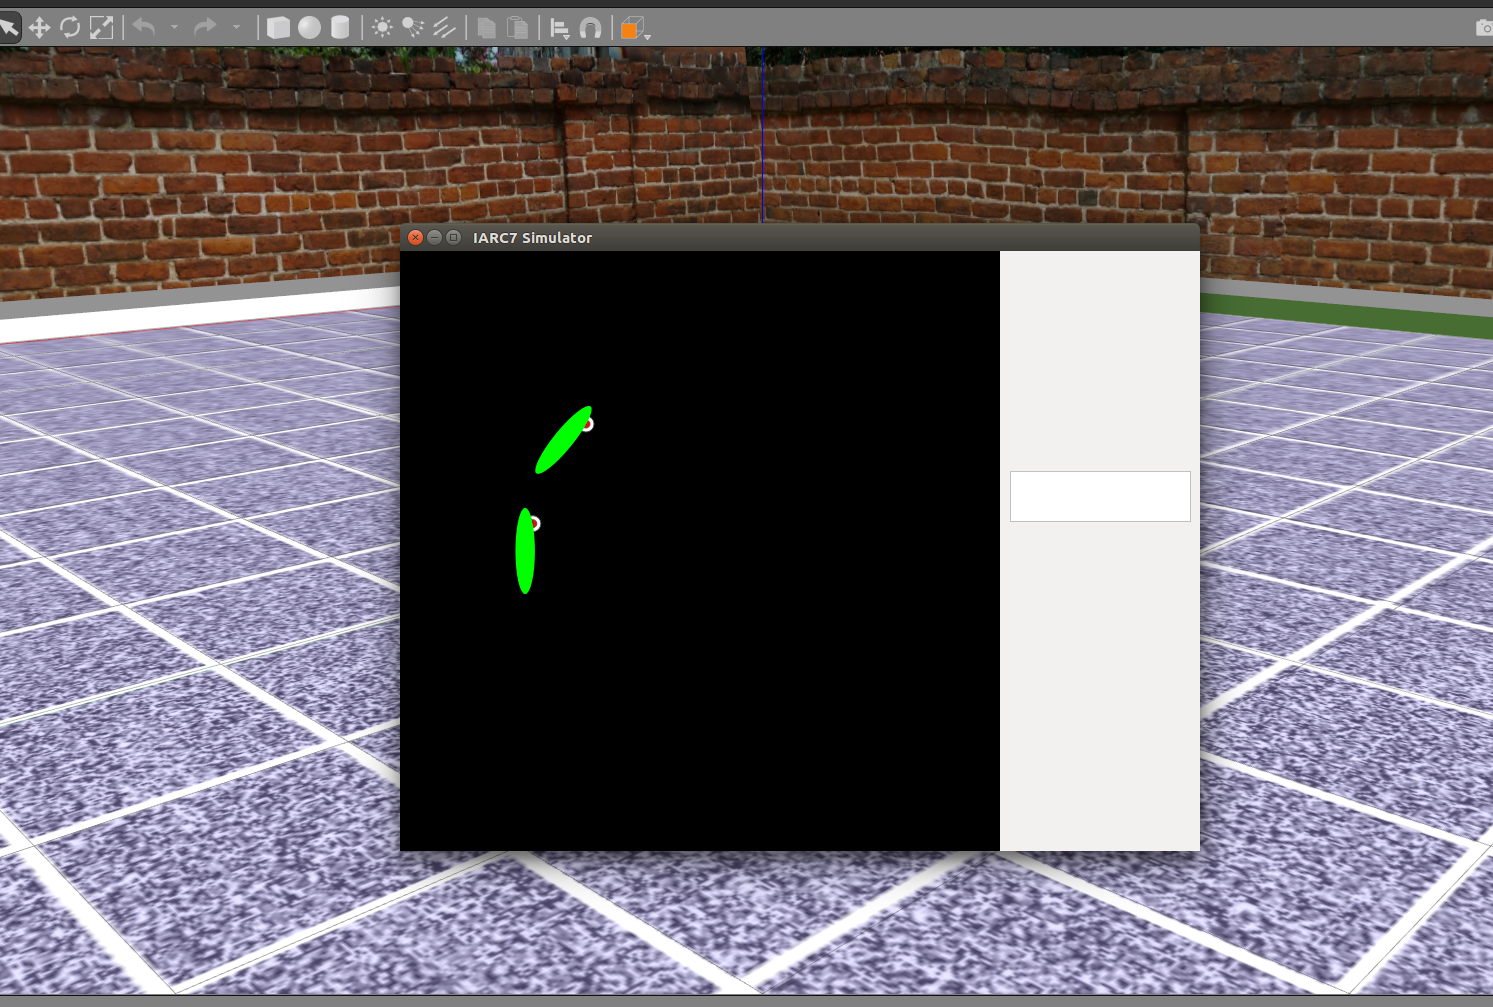
\includegraphics[scale=0.1]{activeloc} \\
    \textbf{Ellipses depicting variance in estimated position of ground bot}\end{center}
    
\subsection{Update Stage}
    
\[ K = PH^{T}(HPH^{T} + R)^{-1}\]
\[ s = f + K(z - Hf)\]
\[ P = (I - KH)P\]
\\
z is the update that we get from the sensor.
\[
h=
  \begin{bmatrix}
    1 && 0 && 0\\
    0 && 1 && 0\\
    1 && 0 && 1\\
  \end{bmatrix}
\]

\[
H=
  \begin{bmatrix}
    1 && 0 && 0\\
    0 && 1 && 0\\
    1 && 0 && 1\\
  \end{bmatrix}
\]

\subsection{Handling Tapping and Collisions}

Collisions are modelled based on the distance between the centers of the error ellipse and the orientation of the ellipse.
If the distance is less than 2 times the bot radius and there is a possibility of head on collision depending on their orientations, we call it a collision and rotate the ellipse by 180 degree. During tapping we simply turn the error ellipse by 45 degree.\\

\section{OBSTACLE AVOIDANCE}
    IARC consists of moving obstacle robots which need to be avoided if they come in the way of the aerial vehicle.
    \\ 
    Obstacles Description: 4 Ground Robots with cylinders attached on top of them to form vertical moving obstacles.
    \\ \\ 
    \textbf{Avoidance Algorithm Overview:} \\
    The Obstacle Avoidance in IARC does not need to be global as the number of obstacles are less in number. So, we use 2-dimensional Lidar attached to a stepper motor to cover 360 degree view for obstacle detection. If the obstacle is closer than a certain threshold then multiple kinds of action can be taken:
    \begin{itemize}
        \item Wait for Obstacle to Move out of Path
        \item Avoid Obstacle by Creating a New Trajectory around the obstacle and come back to desired trajectory.
    \end{itemize}
        \subsubsection*{Procedure I:}
            \begin{itemize}
                \item Interrupt Control is triggered as soon as an obstacle comes closer than 40cm from the Lidar.
                \item Depending on orientation of the obstacle with respect to Lidar and comparing with velocity direction of robot, the robot is halted at the same position or commanded to follow line in reverse till last node is found.
            \end{itemize}}
        \subsubsection*{Procedure II:}
            \begin{itemize}
                \item The hexacopter would follow a biased curved path to reach the destination and at the same time avoid the obstacles.
                \item The path is decided by comparing the angle between the lines joining current position-obstacle position and obstacle position-destination position.
                \item The orientation of the hex is decided by a proportional based controller and is proportional to the difference of the above 2 angles.
                \item Once the distance between hex and destination becomes greater than that between obstacle and destination, go to goal behaviour is resumed.
            \end{itemize}

\section{SYSTEM CONTROL}
\subsection{Pixhawk}
    We have used Pixhawk which runs the PX4 v1.6.0 firmware. PX4 is a nearly feature-complete open source UAV firmware. Thus our high level control utilizes the features of PX4 to its fullest. Since, most of PX4’s autonomous features uses GPS, we use motion capture system to get position data from other sources like vision. Position estimates are sent from an onboard computer. This data is used to update the aerial vehicle's local position estimate relative to the local origin.  
\subsection{MAVROS}
    Since Pixhawk communicates in Micro Air Vehicle Link(MAVLink) protocol and both our ground station and onboard computer uses Robot Operating System(ROS), we used MAVROS for communication between onboard computer and Pixhawk. MAVROS is a MAVLink extendable communication node for ROS.
\subsection{Ground Robot Tapping}
    The MAV is made to do all the required navigation at a default height(say 2.5 metres).For tapping on the ground i-robot, we use a vertical descent strategy.We make our MAV go to a certain calculated location ahead of the ground robot and then make it descend. This calculated position is such that the time required for the ground bot to reach this position is same as the time our MAV would require to descend to the ground robot's height .\\
\\ Assuming a right handed Cartesian coordinate system 
\begin{center}
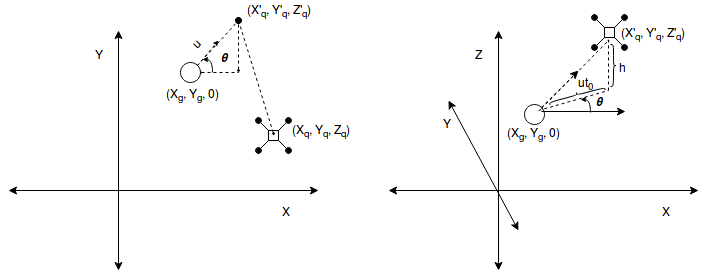
\includegraphics[scale=0.5]{tap}\\
\textbf{Schematic of Tapping}
\end{center}
Let,
    
u = velocity of the ground bot in the direction of its motion 

$\theta$ = orientation of the ground bot with respect to x axis 

$(X_g, Y_g, 0)$ = coordinates of the ground bot 

$(X_q, Y_q, Z_q)$ = Coordinates of the MAV 

($X_q^’$, $Y_q^’$, $Z_q$) = Desired Coordinates of the MAV before it starts to descend 

Where $Z_q$ = $h$ = Default height we want for the MAV in order to avoid obstacles 
        
$t_0$ = time required by MAV to descend from the default height 
 
Calculating the desired coordinates for the MAV, 
 
$X_q^’$ = $X_g + ut_0cos(\theta)$

$Y_q^’$  = $Y_g + ut_0sin(\theta)$ \\
    As soon as the MAV reaches these desired coordinates, it starts descending, vertically. In the same time the ground bot reaches these desired coordinates, making the tap successful. 
    Our only assumption in the method is that the velocity of MAV is greater than the velocity of ground bot. It is ensured by the low level controller that this condition is always satisfied.
\section{IARC ROBOT DESCRIPTION}
\begin{center}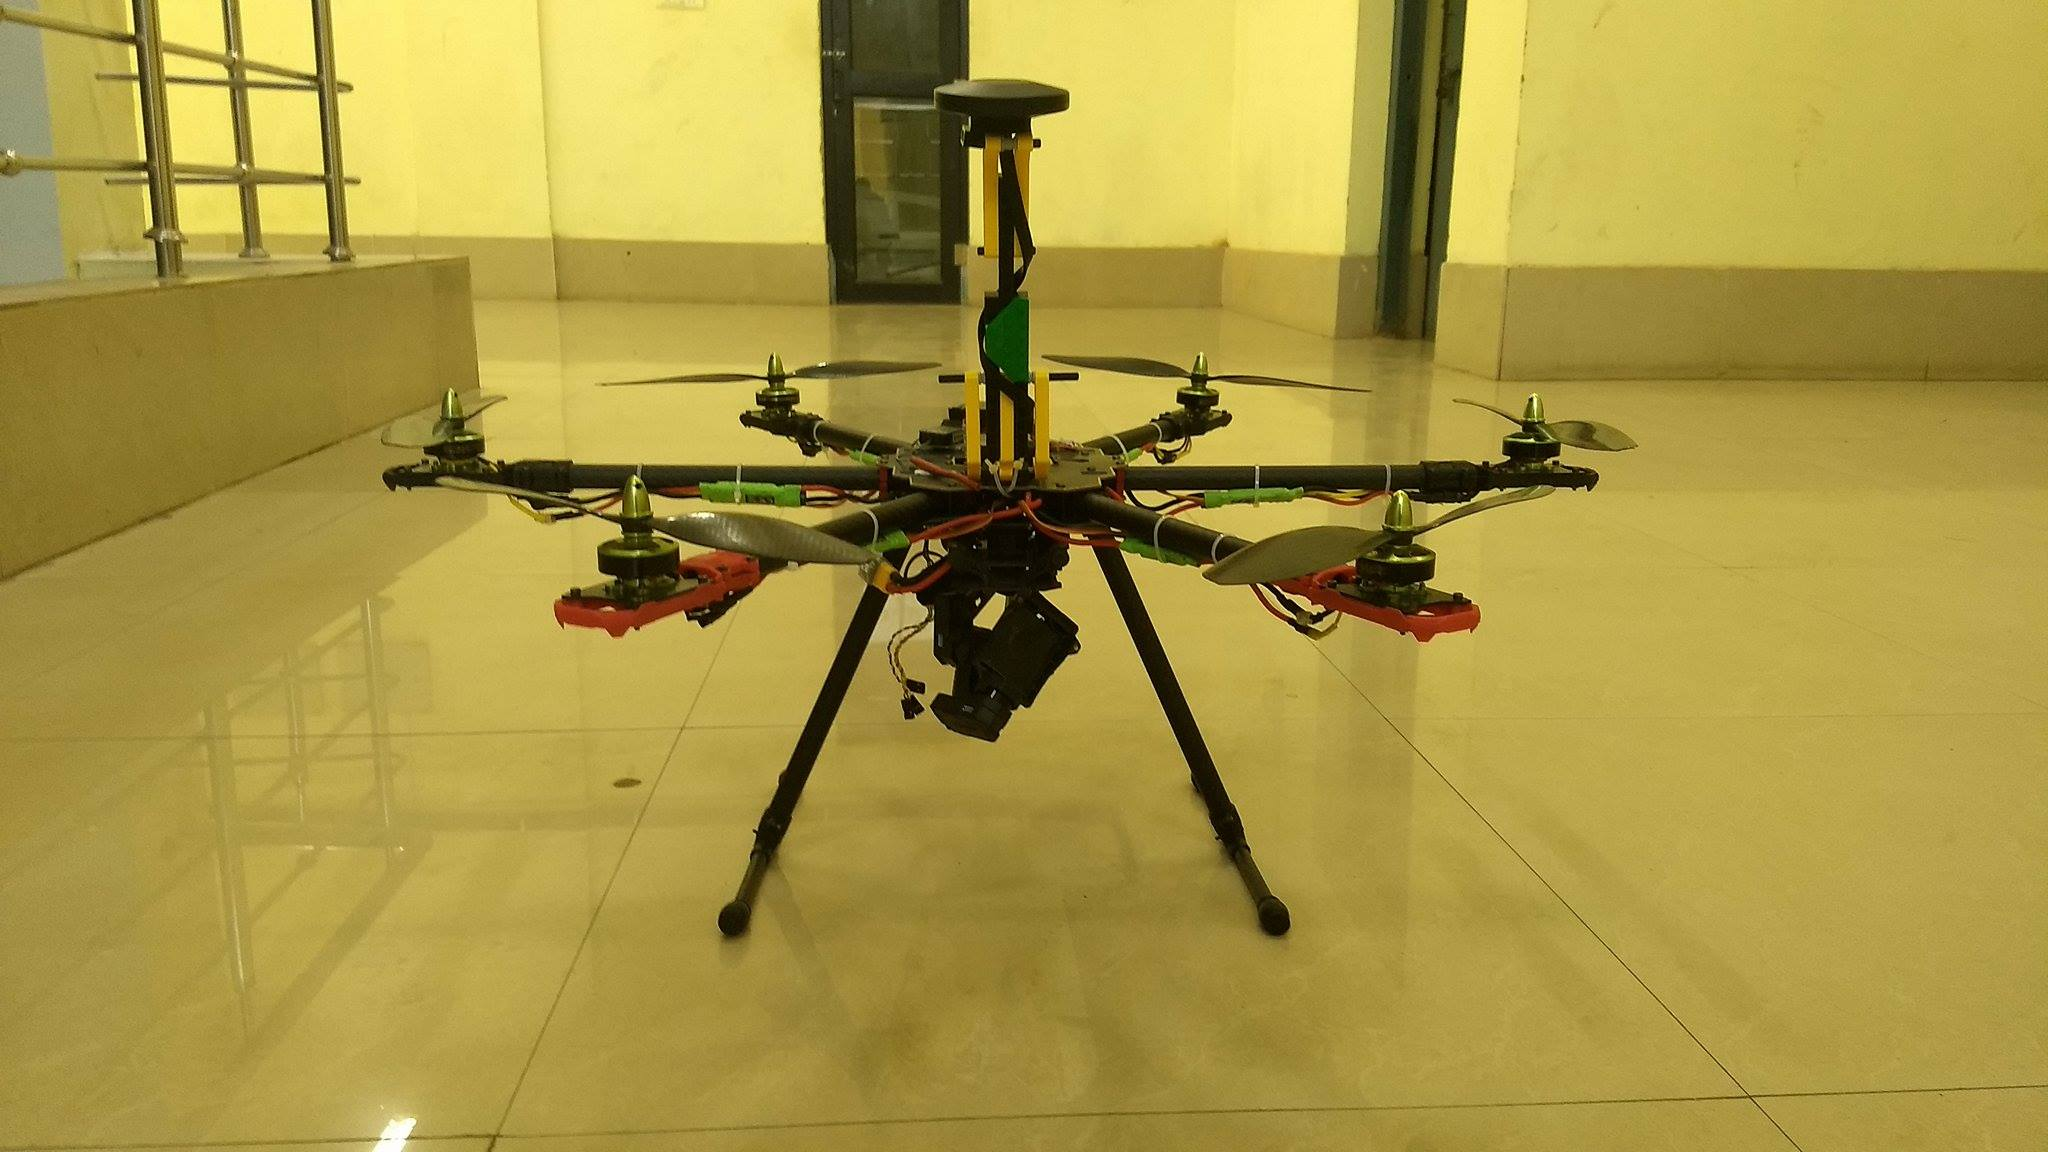
\includegraphics[scale=0.15]{hex} \\
\textbf{Figure 8. Hexcopter}\end{center}\\
\subsection{Configuration}
\begin{itemize}
	\item A carbon-fiber Hex-rotor frame
	\item The stress enduring parts reinforced with PLA 3D printed frames
	\item Customised stands 3D printed using PLA
    \item Odroid XU4 : High Level Controller
    \item Pixhawk : Low Level Controller
    \item Tarot Gimbal T4-3D
    \item ESC     : Electronic Speed Controller, 45A OPTO
    \item LiPo : 14.4V, 4s, 8000mAh, 15C
    \item Motors: 650kv BLDC
    \item Propellers : 12” x 4.5”
    \item 3D printed Tapping plate
    \item Camera Downward: SJ4000
    \begin{itemize}
    	\item Field of View - 78 degrees
    	\item Aspect Ratio - 16:9
    \end{itemize}
    \item Camera Front : Logitech C920
    \begin{itemize}
    	\item Field of View - 78 degrees
    	\item Aspect Ratio - 16:9
    \end{itemize}	
    \item Receiver : 6 channel PPM
    \item Kill switch 
\end{itemize}

	\subsubsection{Hex Frame}
	The main body of the drone is constructed of carbon fiber with custom made base and improvements made using PLA based 3D printed parts. 
	\subsubsection{Motor mounts and other reinforced parts}
	Stress analysis reveals certain places which undergo the maximum stress while take-off and landing. Of those the places which are not made of carbon fiber are reinforced using self designed 3D printed structures. The filament of the 3D printed material uses polylactic acid (PLA), which is a hard plastic.
	\subsubsection{Main stand and Tapping plate}
	The main stand is made out of PLA fixtures and PVC pipes. This stand also embeds in itself a 3D printed tapping plate at its bottom as shown in the picture. 
	\subsubsection{Gimbal and Cameras}
	We are using a Tarot 3-axis gimbal to stabilize the camera feed that we are getting of the wide angle camera. This gimbal is mounted at the front of the hexrotor that faces the camera downwards for the necessary feed.
	\subsection{Emergency Kill Switch}
\begin{itemize}
\item One Dual-D flip flop CD4013B, 5 IRF540N MOSFETs, capacitors and resistors are used. We used the receiver’s signal as source to the circuit which is equivalent to the Pulse generator with variable duty cycle shown in the circuit. The leftmost MOSFET is a controller and the rest 4  mosfets  are connected in series with the negative terminal of LIPO(power source). 4 MOSFET in parallel to each other are used  keeping in mind that each can take a max of around 33 Amps and combined will allow max of around 132 Amps for a quadrotor. For Hexacopter 7 MOSFETs should be used, one as a controller MOSFET and the rest 6(parallel to each other) in series with negative terminal of the power source/LIPO. 6 MOSFETs ensure that max current allowed for the bot is raised to around 190 Amps.  
\item Below a particular duty cycle(T) the controller MOSFET has $V_g_s$<$V_t_h$ and will go in cutoff region as shown below leading zero drain current in it and potential drop across its drain resistor as a result rest MOSFETs will have Vgs=5V due to which they go in saturation region and with very low Vds and in this mode the bot is supplied with power source.\\
\begin{center}
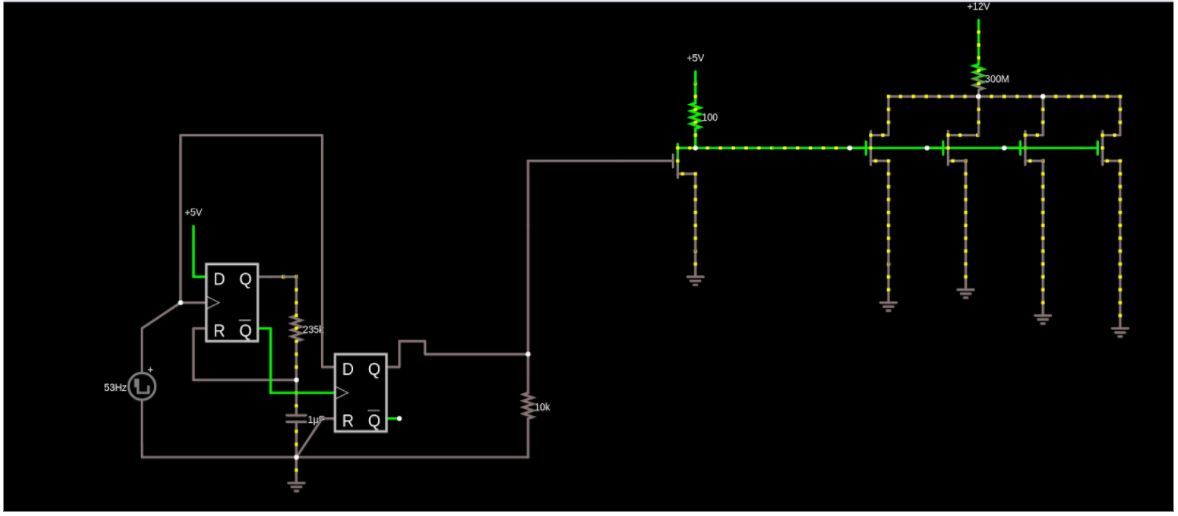
\includegraphics[scale = 0.4]{kill} \\
\textbf{Kill Switch Circuit}\\ \\
\end{center}
\\
\item Above a particular duty cycle(T) the controller MOSFET has $V_g_s$>$V_t_h$ and will go in saturation region and as a result rest MOSFETs will have $V_g_s$ = 0V due to potential drop across drain resistor of controller MOSFET and this will make the rest MOSFETs go in cutoff region as a result cutting off the negative terminal from battery and hence no power supply to the bot. The whole system shuts down instantly.
\item Duty cycle(T) or as in our case PWM of signal  is sent through the transmitter at which the bot is killed can be varied by varying the capacitor’s value.The bot is represented here as the 300 milliohms resistor as there was no way to symbolize the actual bot.
\end{itemize}


\section{HERDING ALGORITHM AI}
\subsection{Greedy Method}
\begin{itemize}
    \item The motif of this algorithm is to make as many bots cross the green line as possible with a fixed radius around the ground bot in which all the other bots will be herd with the centre bot towards the green line.
    \item Once the hexacopter takes off, it will hold altitude at 1.5m (from ground) and hold position on the nearest node while holding its yaw.
    \item The strategy has 3 parts:
    	\begin{itemize}
    		\item Searching
    		\item Following
    		\item Directing (bump or tap)
    	\end{itemize}
    \subsubsection{Searching}
    At the start of the run the quad starts from one of the green line corners. The searching is implemented by
horizontal movement of the quad parallel to the green line. It moves along in a line parallel to the green
line stopping at every 2m to detect any groundbot in its field of view. On reaching the edge it moves
perpendicular to the green line (upwards or downwards) by 1m .
We have considered a rectangular field of view of 5m x 3m . By moving 2m in the parallel direction and 1m
in the perpendicular direction we ensure multiple times overlapping of the visible region to increase the
chances of finding a groundbot.
This searching goes on upward and downward in the arena till we find a groundbot.
Once a groundbot is detected, we lock on the groundbot, let’s say it is called lockedBot and switch to following it.
	\subsubsection{Following}
		Once we get a lockedBot , our aim is to follow it buy always keeping it in our field of view, and keeping
its orientation towards the green line. For this we use the following algorithm:
\begin{itemize}
	\item Follow lockedBot
	\item Continuously check if its orientation - 
		\begin{itemize}
			\item Lies in the correctRegion
			\item Lies in tapRgion
			\item Lies in bumpRegion
		\end{itemize}
	\item Wait if the lockedBot is executing a rotation
\end{itemize}

If, yaw is the orientation of the lockedBot , then, \\

\begin{center}

$yaw \in correctRegion  \ s.t \ yaw  \geq \theta1 \  \&  \ yaw  \leq \theta2$\\ 
$yaw \in tapRegion \ s.t \ yaw  \leq \theta1 \ \& \ yaw  \geq (\theta2 + \pi)$\\
$yaw \in bumpRegion \  s.t yaw \geq \theta2 \  \& \ yaw  \leq (\theta2 + \pi)$\\
  	
\end{center}

where, 

\begin{center}
$\theta1 = atan2(10 - lockedBot.y, 10 - lockedBot.x)$\\
$\theta2 = atan2(10 - lockedBot.y, -10 - lockedBot.x)$\\
\end{center}    

considering, center of the area as origin and y = 10 as the green line.

	\subsubsection{Directing(bump or tap)}
		Once we calculate in which region the orientation lies, corresponding command is given to the quad to do
nothing, bump or tap. \\
When the lockedBot is removed from the green line, we find a nearest node on the grid and start sarching from there, and then algorithm repeats.



\section{TESTING}
\begin{center}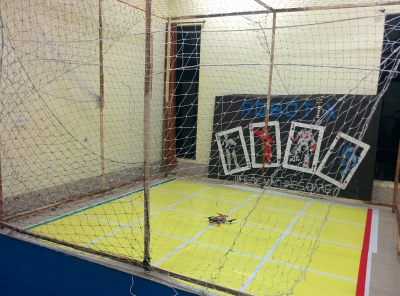
\includegraphics[scale=0.7]{ARK-lab-kgp1} \\
\textbf{Figure 11. Sample testing arena}\end{center}\\
We have an indoor testing arena with sample grid floor as in IARC arena and two iRobots. We have safety harness to 
tie up the quadcopter while testing various controls and PID tuning. \\
We tested the AI (Herding) algorithms on the simulator. We tied the quadcopter with various allowed degree of 
freedom to test altitude hold, yaw hold, node hold and grid following algorithms on the real quadcopter and hexacopter in our arena.
\section{State Machine}
\subsection{States}
\begin{itemize}
\item {Find/ Scan : Quad roams in the arena searching for bots and saving their location.}
\item{Bot Prediction : Predicts the best bot to attack and return its position}
\item{Obstacle Avoidance : Avoids the obstacle}
\item{Strategy : Plans the path and way the bot must be attacked.}
\end{itemize}
\subsection{Working}
\begin{itemize}
\item{Once the take off is successful the control is passed to the FSM. Entry point in the FSM is the Find / Scan state. In find state quad tries to localize itself as well as search for the bot. Detection and localisation is based on probabilistic models including gaussian errors.
}
\item{Quad stays in find state until the probability of bot(s) doesn't increase a certain threshold , let's say K%.
}
\item{Once quad is certain about the position of bot(s) with probability greater than K , control is passed to Bot Prediction state which predicts the bot which should be attacked among the bots with certainty higher than K% and sends the location of the bot to Strategy state.
}
\begin{center}
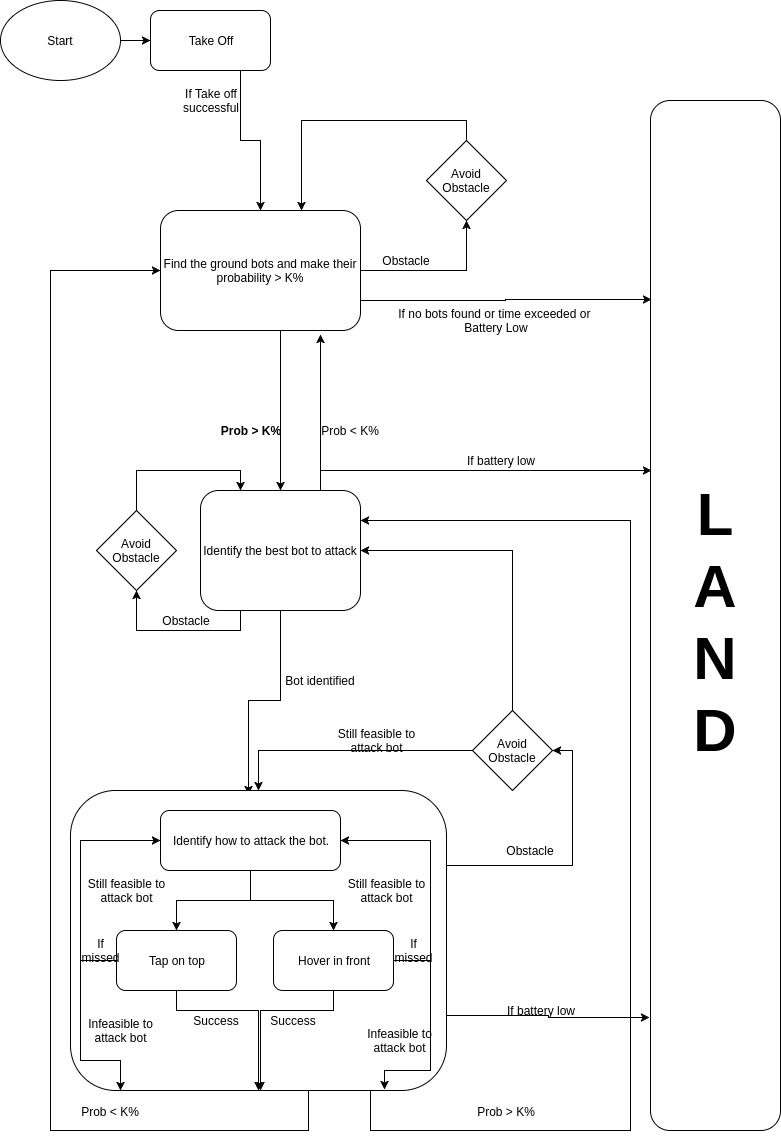
\includegraphics[scale=0.4]{st_mcn} \\
\textbf{State Machine Diagram}\end{center}\\
\item{Strategy state tries to analyze the different states of the bot like position, velocity and direction and accordingly decides how the particular bot should be attacked.
}\\
If any of the two method fails to execute properly and the probability of the current bot is still high and feasible to attack the state is looped to re-determine the best way among two to again attack the bot, else control simply shifts to bot prediction mode to identify the next best bot to attack.
\end{itemize}
\subsection{Rules}
\begin{itemize}
\item{State interrupted is re-run after obstacle is avoided excluding the Strategy state where a check redirects it to Strategy or Bot detection state according to the feasibility of attacking the same bot again.
}
\item{Anytime the probability of bot(s) go below the K, state will shift to Find / Scan to increase the certainty of the bot(s). Exceptions :
}
\begin{itemize}
\item{Quad is attacking one bot with high certainty : A threshold delta must be considered in such conditions when the probability of other bots is allowed to fall as low as K-delta % as attacking the bot may increase our points.
}
\end{itemize}
\item{Battery is given the highest priority of all. If the battery is low , state machine will be terminated and the quad will land.
}
\end{itemize}
\section{References}
\begin{enumerate}
        \item \href{https://books.google.co.in/books?id=4YCThwzeTBQC&redir_esc=y}{\textit{E. L. Houghton, P.W.Carpenter} Aerodynamics for Engineering Students. 
    \item \href{https://books.google.co.in/books/about/Fundamentals_of_Aerodynamics.html?id=CaBTAAAAMAAJ}{$\textit{John David Anderson}$ Fundamentals of Aerodynamics. }}
    \item \href{https://books.google.co.in/books/about/Fundamentals_of_Compressible_Flow.html?id=_NCz9iZIugYC}{\textit{S. M. Yahya } Engineer's Aerodynamics. }
    \item \href{https://ieeexplore.ieee.org/document/8115889/}{\textit{Manash Pratim Das, Gaurav Gardi, Jayanta Mukhopadhyay} 5-DoF monocular visual localization over grid based floor}
    \item \href{http://eprints.qut.edu.au/33732/1/cep2009_modelling_and_control_paper_sub_final.pdf}{\textit{P. Pounds, R. Mahony, and P. Corke} Modelling and Control of a Large Quadrotor Robot. }
    \item \href{http://ieeexplore.ieee.org/iel5/5076472/5152175/05152390.pdf?arnumber=5152390}{\textit{P. Pounds and R. Mahony} Design principles of large quadrotors for practical applications. }
    \item \href{https://www.researchgate.net/publication/220474158_Towards_autonomous_indoor_micro_VTOL}{\textit{Samir Bouabdallah, Samir Bouabdallah and Roland Siegwart} Towards autonomous indoor micro VTOL. }
    \item \href{http://www.itcon.org/cgi-bin/works/Show?2012_12}{ \textit{Javier Irizarry, Masoud Gheisari and Bruce N. Walker, Associate} Usability assessment of drone technology as safety inspection tools.}
    \item \href{http://www.engadget.com/2011/04/21/t-hawk-uav-enters-fukushima-danger-zone-returns-with-video/}{ T-Hawk UAV enters Fukushima danger zone, returns with video. 6:48PM April 21, 2011, retrieved on April 22, 2011.}
    \item \href{http://9to5mac.com/2011/06/15/awesome-use-of-an-ipad-and-the-parrot-ar-drone/}{\textit{Zibreg. C. (2011)} Awesome use of an iPad and the Parrot AR Drone. }
    \item \href{http://robotics.felk.cvut.cz/faiglj/thesis/papers/icr10.pdf}{\textit{Jan Faigl,  T Krajnık,  V Vonásek,  L Preucil} Surveillance Planning with Localization Uncertainty for UAVs.}
    \item \href{http://ieeexplore.ieee.org/xpl/articleDetails.jsp?reload=true&arnumber=6005280}{ \textit{Wai Shan Ng and Ehud Sharlin} Collocated interaction with flying robots.} 
    \item \href{https://www.researchgate.net/publication/220947254_Flying_sports_assistant_External_visual_imagery_representation_for_sports_training}{\textit{Higuchi, K., Shimada, T., and Rekimoto, J.} Flying sports assistant: external visual imagery representation for sports training.}
    \item \href{http://www.aviationsystemsdivision.arc.nasa.gov/publications/hitl/rtsim/Toms.pdf}{\textit{T. S. Alderete, NASA Ames Research Center, Moffett Field, California.} Simulator aero model implementation.}
    \item \href{https://www.researchgate.net/publication/228962656_Nonlinear_observer_design_and_sliding_mode_control_of_four_rotor_helicopter}{ \textit{ H. Bouadi and M. Tadjine} Nonlinear observer design and sliding mode control of four rotors helicopter.}
    \item \href{https://april.eecs.umich.edu/papers/details.php?name=olson2010tags}{\textit{Edwin Olson} AprilTag: A robust and flexible multi-purpose fiducial system.}
    \item \href{https://pjreddie.com/darknet/yolo/}{\textit{Redmon, Joseph and Farhadi, Ali (2016)} YOLO9000: Better, Faster, Stronger \textit{arXiv preprint arXiv:1612.08242}}
    \item \href{http://www.cse.psu.edu/~rtc12/CSE486/lecture12.pdf}{\textit{Robert Collins, CSE486, Penn State} Lecture 12: Camera Projection}
    \item \href{http://wiki.ros.org/px4flow_node}{px4flow\_node}
    \item \href{https://github.com/RoboJackets/hungarian}{Github: RoboJackets/hungarian}
    \item \href{http://quadrotor-iitkgp.github.io/}{Aerial Robotics Kharagpur: Website}
    \item \href{https://github.com/quadrotor-IITKgp}{ Aerial Robotics Kharagpur: GitHub organization}

\end{enumerate}
\end{document}
